\chapter{Introduction\label{ch:intro}}

\graphicspath{{figs/introduction/}}

The brain is a truly remarkable machine. It routinely performs tasks that are impossible for even the most powerful supercomputer, and it does so in a highly energy-efficient manner. It can analyze patterns extremely efficiently, interpret them, and produce appropriate behavioral responses. It can store enormous amounts of information, allowing us to recollect things like phone numbers, familiar faces, songs and episodes from early life. But perhaps even more impressively, the brain is capable of producing consciousness, and allows us to experience our own thoughts and feelings. 

Scientists' desire to unlock the mysteries of the brain is obvious. Not only would it allow us to better understand, and perhaps cure, the hundreds of different brain diseases that exist, such as depression, Alzheimer's disease, Parkinson's disease, epilepsy, and migraine. The knowledge of how the brain solves complex problems would likely also result in radical changes to how computers work. New storage technologies that mimic the way the brain stores and recollects memories might emerge, and computers might finally be able to learn the way humans do. Artificial intelligence (AI) might seem a lot less artificial. 

However, understanding the brain is one of the greatest challenges facing scientists today. A great deal is understood about how single neurons function, how they communicate with other neurons through synapses, and how these synapses are formed and change over time. What is not well understood is how brain function emerges from billions of neurons communicating with each other over trillions of synapses. One way to address this problem is to simulate the activity of a large number of neurons in a computer. With such a simulation, the effects of small changes in neurons and synapses on the dynamics of large networks can be studied. The Human Brain Project (HBP), recently awarded one billion euros by the European Commission \cite{abbott2013brain}, aims to simulate a full scale human brain within a decade \cite{hbp2012}. With this flagship project engaging and inspiring the scientific community, the importance of simulations in brain science is likely to continue to increase in the years to come. 

A number of neural network simulators are available, such as NEURON, GENESIS, Brian, and NEST \shortcite{Bret:2007(349)}. This thesis will focus on NEST \shortcite{Gewaltig:NEST}, a popular simulation environment for simulating large networks of point neurons.
As scientists are increasingly relying on tools like these to make new discoveries, the need for quality checking of the software increases. There is always a chance that a mistake has crept into a piece of computer code, one that does not make the program crash, but causes erroneous scientific results. In a famous example, a paper detailing the structure of a protein called MsbA \shortcite{Chang07092001}, had to be retracted because the reported structure turned out to be wrong. The reason for the incorrect result was that two columns of data were flipped in the computer program that derived the protein structure \shortcite{Miller22122006}. It took more than five years before the mistake was detected, and by that time the paper had been cited by 364 publications, according to Google Scholar. Four other papers also had to be retracted due to the same malfunctioning computer program. 

%%%%%%%%%%%%%%%%%%%%%%
% Testing in general %
%%%%%%%%%%%%%%%%%%%%%%

A good way to detect these kinds of mistakes in computer code is through unit testing. The idea here is to divide the program into small units that can be tested rigorously by comparing the units output with our expectations \cite{huizinga2007automated}. While this approach has its merits, tests will not be able to detect all conceivable error that could occur. In the words of \shortciteN{dijkstra1970notes}, ``Program testing can be used to show the presence of bugs, but never to show their absence!''.

%%%%%%%%%%%%%%%%%%%%%%%%%%%%%%%%%%%%%%%%%%%%%%%%%%%%%%%%%%%%%
% Additional challenges when testing probabilistic programs %
%%%%%%%%%%%%%%%%%%%%%%%%%%%%%%%%%%%%%%%%%%%%%%%%%%%%%%%%%%%%%

When testing probabilistic algorithms using statistical tests, some additional challenges arise. For instance, the tests will occasionally give false positives, i.e., they will report a problem with the tested algorithm where none exists. One can not get completely rid of false positives, but strategies can be devised to reduce the frequency with which they occur. Statistical tests will also give false negatives, i.e., they will fail to report true problems. Again, this is unavoidable, all we can do is to try to increase the sensitivity of the tests, i.e., their ability to detect problems. This ties in with a more general problem; that of testing randomness. 

To generate a sequence of seemingly random numbers, computer software relies on pseudorandom number generators PRNGs \shortcite{Lecu:2004(35)}. The sequences they produce is not truly random, but generated by a deterministic algorithm (hence the prefix ``pseudo''). For most applications, however, the numbers are sufficiently unpredictable as to be considered random, depending on the specific algorithm used and how it is implemented. There are several ways to test the output of a PRNG. One approach is to look for a systematic bias by comparing the expected distribution of numbers with an observed sample distribution using some goodness-of-fit (GOF) test, such as the Kolmogorov-Smirnov (KS) test or the Anderson-Darling (AD) test, but this approach will not detect other kinds of patterns such as clustering of the produced numbers, as long as the clusters are distributed relatively evenly. Other methods may pick up such clustering, but yet other unforeseeable patterns might still go undetected. As argued by \citeN{lecuyer2007testu01}, no statistical test or battery of tests can guarantee that the output of a PRNG will be sufficiently random under all circumstances. Some application might cause some structure to emerge due to an artifact of the PRNG's algorithm. 

When testing probabilistic algorithms using statistical tests, we are faced with the same problem. No statistical test or battery of tests can prove beyond any doubt that the algorithm is without biases or patterns that affects the output of a computer program. Still, the more tests the algorithms can pass, the greater our confidence in them, and hence the scientific findings based on them. 

%%%%%%%%%%%%%%%%%%%%%%%%%%%%%%%%%%%%%%%%%%%%%%%%%%%%%%%%%%%%
% What you specifically want to test (connection patterns) %
%%%%%%%%%%%%%%%%%%%%%%%%%%%%%%%%%%%%%%%%%%%%%%%%%%%%%%%%%%%%

\subsection*{Connectivity patterns in neuronal network models}
\markright{Connectivity patterns in neuronal network models} 

A neural network can be described as a directed, weighted graph where the nodes are neurons, or sometimes devices, and the edges are connections or synapses between them. Events can be transmitted in one direction over the connections. These events are action potentials (spikes) or other types of signals that can be transmitted over synapses.

In any type of network modeling, the network structure must be specified. In principle, this could be done by listing all the nodes and their connections. This kind of specification, however, is not very manageable for us humans. To be able to work with network models, discuss them, and share them, higher-level descriptions of connection patterns are needed. Populations of nodes can then be connected following some basic rules to create these patterns. Ways to unambiguously describe and document connection patterns have been lacking, but recent efforts have been made to standardize their terminology and notation \shortcite{nordlie2009visualizing,djurfeldt2012connection,crook2012creating}. Since NEST is used in this thesis, we will mainly use NESTs terminology. We will now describe the relevant connection patterns and related concepts and terminology. 

A {\bf random divergent connection} between a source population and a target population is defined as the connection pattern resulting from connecting each node in the source population to a prescribed number $C$ of randomly drawn target nodes. An example of this kind of network is shown in Figure \ref{fig:rdc_example_intro}.
\begin{figure}[b]
  \centering
  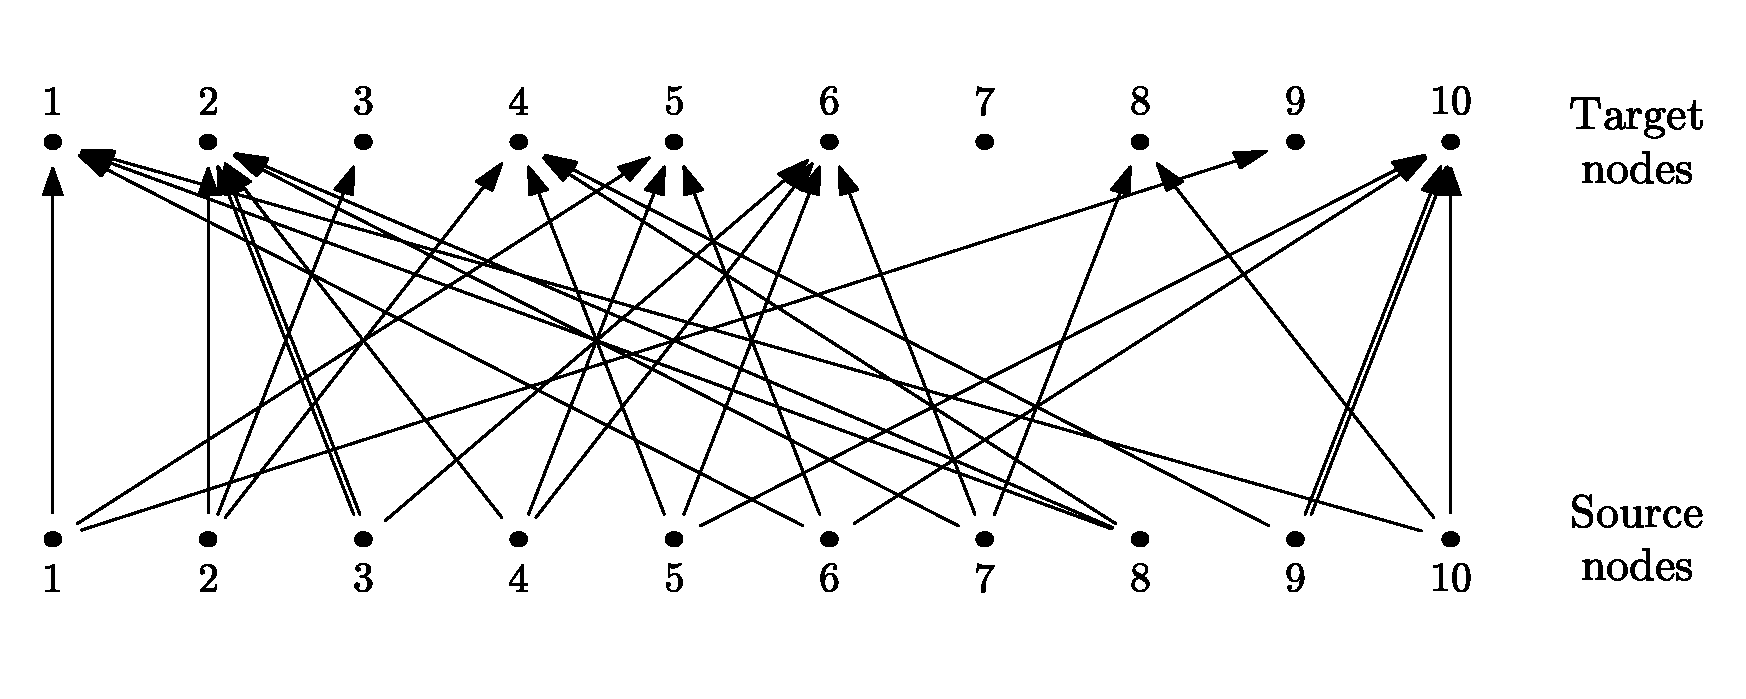
\includegraphics[width=\textwidth]{RandDivConn.pdf}
  \caption[A random divergent connection pattern]{Example of how a random divergent network might look. All source nodes have an out-degree of 3, while the target nodes have different in-degrees.}
  \label{fig:rdc_example_intro}
\end{figure}
The target nodes are drawn with replacement, meaning multiple connections can exists between any pair of nodes (multapses). If the source and target populations are the same population, nodes will also be able to connect to themselves (autapses). It is possible to disallow multapses and autapses in NEST, but we will assume they are allowed. 

In a {\bf random \emph{convergent} connection}, $C$ \emph{source nodes} are randomly drawn, with equal probability, for each target node. The in-degree is now $C$ for all target nodes, while the source nodes might have different out-degrees.

Network models can also have spatial structure. In such models, connection probabilities, as well as connection properties such as weight and delay, can be a function of the distance between the source and the target node. In this way, connectivity patterns that mimic observed axonal projection patterns can be created. Thus, when referring to a {\bf spatially structured network} in this thesis, we mean a network whose connection probabilities depend on source-target distance. In spatially structured networks, populations of nodes can exist in two- or three-dimensional space. The distance-dependent connection probability function is referred to as the {\bf kernel}. Only nodes inside an area or volume called the {\bf mask} are eligible connection targets. The location of the mask is usually given relative to the node considered. A two-dimensional spatially structured network is shown in Figure \ref{fig:spatial_example_intro}, where a square mask and a Gaussian kernel are used.

\begin{figure}[h]
  \centering
  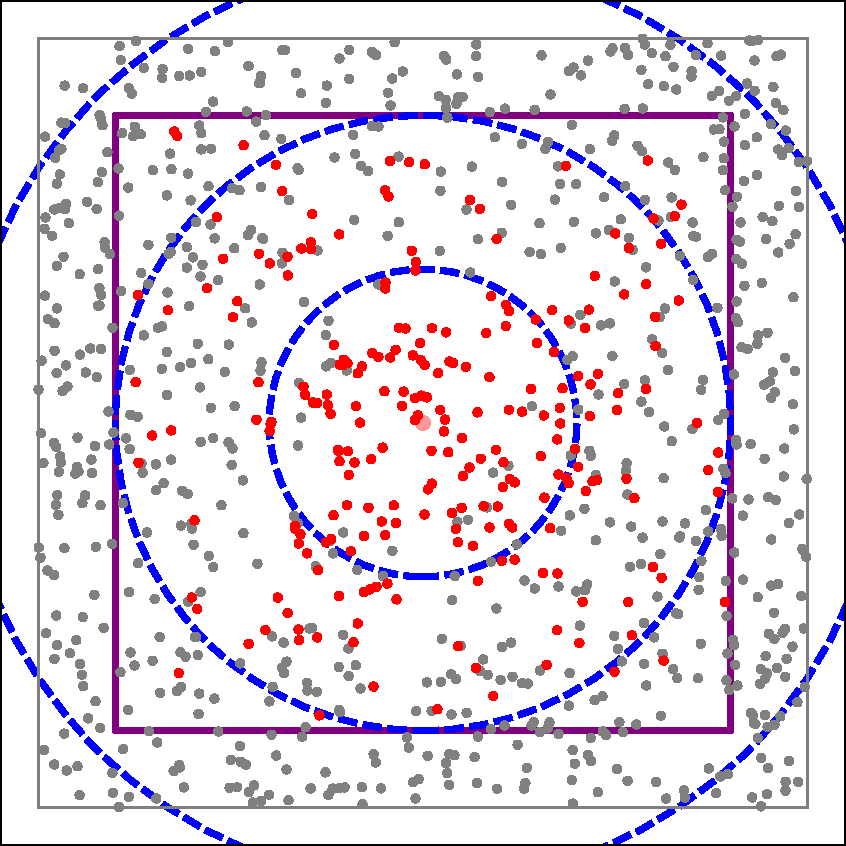
\includegraphics[width=0.6\textwidth]{TopologyExample3D.pdf}
  \caption[A spatially structured network]{Example of how a spatially structured network might look. 1,000 nodes are scattered across the layer. The centered source node is connected to the red nodes, but not the grey. The mask is shown in purple, and the blue rings mark $\sigma$, $2\sigma$ and $3\sigma$ from the Gaussian kernel. }
  \label{fig:spatial_example_intro}
\end{figure}



\subsection*{Aims and organization of this thesis}
\markright{Aims and organization of this thesis}

The aim of this thesis is to develop statistical tests for the probabilistic connection algorithms used in neural network simulators, both for networks with and without spatial structure. Further, an automated test suite that can run relatively quickly, with a low rate of false positives, possibly as part of the automated testing in a continuous integration system, is developed. To demonstrate the utility of the test procedures, they are used to test the connection algorithms of NEST. It is worth emphasizing that the test suites can easily be modified to work with data obtained from any other simulator that shares the basic connection schemes. 

Chapter \ref{ch:statistical} will start with a short introduction to the statistical tests that will be used later, and introduce the concept of a two-level test procedure. In Chapter \ref{ch:nonspatial}, a test procedure for random connections with predefined in- or out-degree is developed. NEST-specific implementations are discussed, and results are presented, both for convergent (Section \ref{sec:rcc}) and divergent (Section \ref{sec:rdc}) connections. In Section \ref{sec:auto}, an automated test procedure is proposed and implemented for NEST.

Networks with spatial structure are discussed in Chapter \ref{ch:spatial}. Test strategies are developed and implemented for NEST, and results are presented, first for two-dimensional space in Section \ref{sec:2D}, then for three dimensions in Section \ref{sec:3D}. A general discussion about findings and perspectives for future research is found in Chapter \ref{ch:disc}.

As the tests proposed in this thesis are implemented for NEST, there will be references to functions in NEST. The reader might therefore want to take a look at the NEST tutorial found in Appendix \ref{app:nest} before proceeding. 



\clearchapter

